%----------createAssociationBetweenClasses----------------------------------------
\op
{createAssociationBetweenClasses}
{creates a new association between classes}
{createAssociationBetweenClasses(Package selectedEObject, String nameValue,
String idValue, String srcMultiplicity)} {The package providing the container
for the newly created association.} {
\begin{itemize}
 \item nameValue/newName: The name of the newly created association
 \item idValue/newID: The id of the newly created association
 \item srcValue/newSrcName: The name of the newly created source association end
 \item srcIdValue/newSrcID: The id of the newly created source association end
 \item srcMultiplicity/newMultiplicity: The multiplicity of the newly created
 source association end
 \item tgtValue/newTgtName: The name of the newly created target association end
 \item tgtIdValue/newTgtID: The id of the newly created target association end
 \item tgtMultiplicity/newMultiplicity: The multiplicity of the newly created
 target association end
\end{itemize}
}
{The 'newSrcName' and 'newTgtName' must differ (see
\ref{subsec:checkOtherNames})}
{This rule firstly creates an association under the propagated package with
input data for id and name. Secondly it will create association ends with input data for id, name and
multiplicity (isNavigatable, kind and isOrdered will recieve default
values). Afterwards it will append them to the association created beforehand
via references (association and associationEnds). Lastly the association
ends will either get a reference (target) to an input class.
\\Note that the reference from a class and from the selected association point to
the same unknown package. This will make sure that there won't be created
associations between classes of different packages.}
\begin{figure}[H]
  \centering
  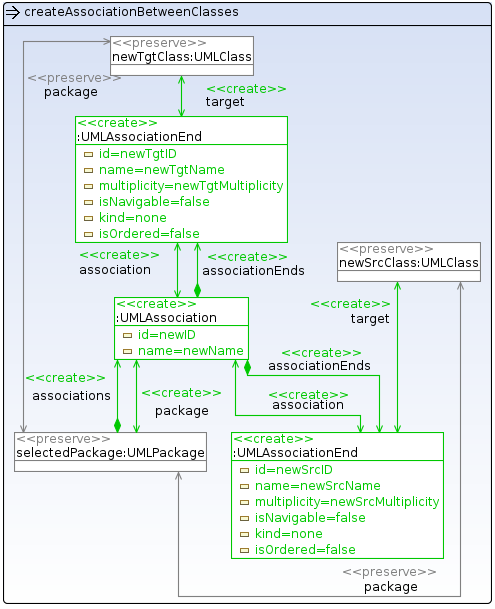
\includegraphics[width=0.8\textwidth]{pics/createAssociationBetweenClasses.png}
  \caption{createAssociationBetweenClasses}
  \label{createAssociationBetweenClasses}
\end{figure}
%----------createAssociationBetweenInterfaces----------------------------------------
\op
{createAssociationBetweenInterfaces}
{creates a new association between interfaces}
{createAssociationBetweenInterfaces(Package selectedEObject, String nameValue,
String idValue, String srcMultiplicity)} {The package providing the container
for the newly created association.} {
\begin{itemize}
 \item nameValue/newName: The name of the newly created association
 \item idValue/newID: The id of the newly created association
 \item srcValue/newSrcName: The name of the newly created source association end
 \item srcIdValue/newSrcID: The id of the newly created source association end
 \item srcMultiplicity/newMultiplicity: The multiplicity of the newly created
 source association end
 \item tgtValue/newTgtName: The name of the newly created target association end
 \item tgtIdValue/newTgtID: The id of the newly created target association end
 \item tgtMultiplicity/newMultiplicity: The multiplicity of the newly created
 target association end
\end{itemize}
}
{The 'newSrcName' and 'newTgtName' must differ (see
\ref{subsec:checkOtherNames})}
{This rule firstly creates an association under the propagated package with
input data for id and name. Secondly it will create association ends with input data for id, name and
multiplicity (isNavigatable, kind and isOrdered will recieve default
values). Afterwards it will append them to the association created beforehand
via references (association and associationEnds). Lastly the association
ends will either get a reference (target) to an input interface.
\\Note that the reference from an interface and from the selected association
point to the same unknown package. This will make sure that there won't be created
associations between interfaces of different packages.}
\begin{figure}[H]
  \centering
  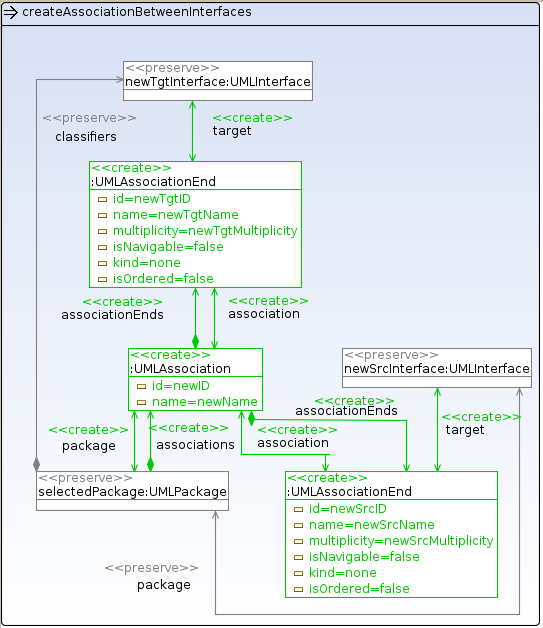
\includegraphics[width=0.8\textwidth]{pics/createAssociationBetweenInterfaces.png}
  \caption{createAssociationBetweenInterfaces}
  \label{createAssociationBetweenInterfaces}
\end{figure}
%----------deleteAssociation----------------------------------------
\op
{deleteAssociation}
{Deletes an association}
{deleteAssociation(Association selectedEObject)}
{The association which should be deleted including all its containments and all
its references}
{-}
{-}
{For this transformation three rules are needed. The first two will be used to
delete the target reference of an association end depending on the type of
the target. The third rule will delete the selected association from its
container package.
\\In the second picture you can find the TransformationUnits. It contains a
Sequential 'mainUnit' which will firstly run the Counted Unit
'LOOP\_deleteAssociationEndIsClass'. After there is no associaton end under the
selected association left which points to a class, the next Counted Unit
'LOOP\_deleteAssociationEndIsInterface' will be run. Both Counted Units behave
similarily. When there are no available association ends left, the
deleteAssociation-Rule will be called.}
\begin{figure}[H]
  \advance\leftskip-1.5cm
  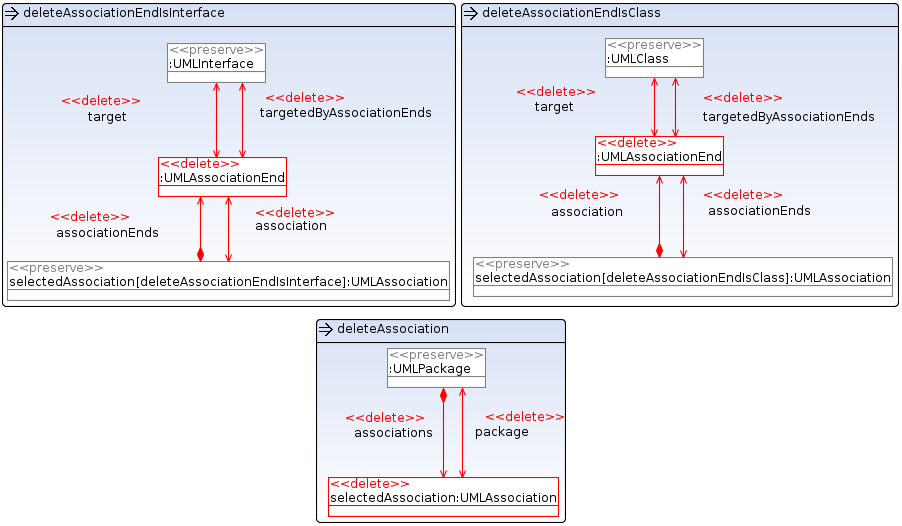
\includegraphics[width=1.2\textwidth]{pics/deleteAssociation.png}
  \caption{deleteAssociation}
  \label{deleteAssociation}
\end{figure}
\begin{figure}[H]
  \advance\leftskip-1.5cm
  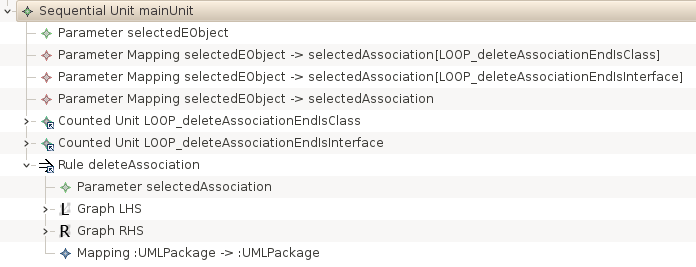
\includegraphics[width=1.2\textwidth]{pics/deleteAssociation_TreeView.png}
  \caption{deleteAssociation(UnitView)}
  \label{deleteAssociation(UnitView)}
\end{figure}
%----------editAssociationName----------------------------------------
\op
{editAssociationName}
{edits the name of an association}
{editAssociationName(Association selectedEObject, String nameValue)}
{The association whose name should be renamed.}
{
\begin{itemize}
 \item nameValue/newName: The new name
\end{itemize}
}
{-}
{The \textless\textless create\textgreater\textgreater  -symbol in the image
means that even if the attribute exists its value will be overwritten.
'newName' is the placeholder for the input name.}
\begin{figure}[H]
  \centering
  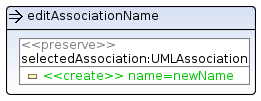
\includegraphics[width=0.45\textwidth]{pics/editAssociationName.png}
  \caption{editAssociationName}
  \label{editAssociationName}
\end{figure}